%%%%%%%%%%%%%%%%%%%%%%%%%%%%%%%%%%%%%%%%%%%%%%%%%%%%%%%%%%%%%%%%%%%%%%%%%%%%%
\chapter{Konzept}
\label{chap:concept}
%%%%%%%%%%%%%%%%%%%%%%%%%%%%%%%%%%%%%%%%%%%%%%%%%%%%%%%%%%%%%%%%%%%%%%%%%%%%%
\chapterstart

Um eine Optimierung der Skalierbarkeit sowie der Ressourceneffizienz eines Web-Crawlers durchzuführen, ist eine fundierte Konzeptionierung essenziell. Im nachstehenden Kapitel wird auf traditionelle Web-Crawling Konzepte eingegangen. Diese werden beleuchtet und wichtige Erkenntnisse zusammengefasst, die im Folgenden in die Konzeption einer optimierten Variante einfließen. 

Im Subkapitel \textit{\nameref{sec:cloudnative}} werden zunächst Konzepte zur Unterstützung der Hypothese \textit{\nameref{subsec:hypothesis:scalability}} untersucht. Das Kapitel gibt einen Überblick über die Cloud-native Landschaft und ihren Prinzipien. Mit diesen Erkenntnissen wird in Kapitel \ref{subsec:microservicekontextcrawler} eine Optimierung eines traditionellen Web-Crawling Ansatzes durchgeführt.

Das darauffolgende Kapitel, betitelt als \textit{\nameref{sec:aot}}, befasst sich mit dem Konzept der \ac{AOT} und dessen Bedeutung in Bezug auf die Verbesserung von Web-Crawling Methoden. Zunächst wird die Definition der \acl{AOT} vorgestellt, gefolgt von einer detaillierten Gegenüberstellung dieser mit der \acl{JIT}. Diese Gegenüberstellung ermöglicht eine tiefgreifende Analyse der Vor- und Nachteile beider Ansätze. Abschließend wird untersucht, wie die \acl{AOT} spezifisch in den Web-Crawling Kontext integriert werden kann, um die Leistung und Effizienz des Crawling-Prozesses zu verbessern.
\section{Traditionelle Web-Crawling Konzepte}\label{sec:traditionalconcepts}
Im Bereich des Web-Crawling existieren verschiedene Techniken, die dazu dienen, spezifische Herausforderungen in diesem Bereich erfolgreich zu bewältigen. Einige der Herausforderungen, denen Web-Crawling gegenübersteht, könnten beispielsweise die effiziente Verwaltung von großen Datenmengen, die Überwindung von Zugriffsbeschränkungen auf bestimmten Webseiten, die Erkennung und Handhabung von dynamisch generierten Inhalten sowie die effektive Navigation durch komplexe Strukturen von Webseiten sein. 

Eine allgemeine Unterteilung definiert das Werk \citetitle{sharma2015anatomy}~\parencite[vgl.][S. 1-3]{sharma2015anatomy}{}{}. In diesem Werk werden vier verschiedene Typen von Web-Crawlern erwähnt und miteinander verglichen, welche nachstehend erläutert werden:

\begin{itemize}
    \item \textbf{Parallel-Crawlers}: Diese Crawler arbeiten gleichzeitig mit mehreren Instanzen, um große Teile des Web effizient zu durchsuchen.
    \item \textbf{Focused-Crawlers}: Diese sind auch bekannt als ''Thematische-Crawler'' oder ''Topical-Crawler'' und konzentrieren sich vor allem auf spezifische Inhalte oder Themengebiete. Durch den Einsatz von Klassifikatoren und die Priorisierung von Links, die zu themenrelevanten Ressourcen führen, verbessern sie die Effizienz der Datensammlung in Bezug auf ein spezifisches Interessengebiet.
    
    \item \textbf{Incremental-Crawler}: Diese Crawler zielen darauf ab, die bereits untersuchten Inhalte aktuell zu halten, indem sie das Web kontinuierlich durchsuchen und periodisch bereits untersuchte Seiten erneut besuchen. Sie berücksichtigen die Änderungshäufigkeit und Wichtigkeit der Seiten.
    
    \item \textbf{Hidden-Crawler}: Sie sind darauf spezialisiert, Inhalte zu erfassen, welche hinter Suchformularen oder Bereichen verborgen und durch bereits erwähnte Web-Crawler nicht erreichbar sind. Diese Crawler interagieren mit Webformularen und sammeln Daten aus Datenbanken, die erst nach einer Formularübermittlung zugänglich werden.
\end{itemize}

Durch die gezielte Anwendung dieser Techniken lassen sich diverse Ansätze für eine Architektur ableiten. Im speziellen Kontext des Web-Crawlings ist das übergeordnete Ziel stets die Entwicklung eines höchst optimierten Architekturansatzes. Hierbei spielen Effizienz, Leistungsfähigkeit und Skalierbarkeit eine zentrale Rolle. Es gilt, eine Architektur zu gestalten, die den spezifischen Anforderungen des Web-Crawlings gerecht wird und dabei maximale Effektivität gewährleistet.
\newline
In der Regel beruhen Crawling-Systeme auf einem gemeinsamen Grundprinzip, welches in Abbildung \ref{fig:architecture-general} visualisiert wird.
\begin{figure}[H]
    \centering
    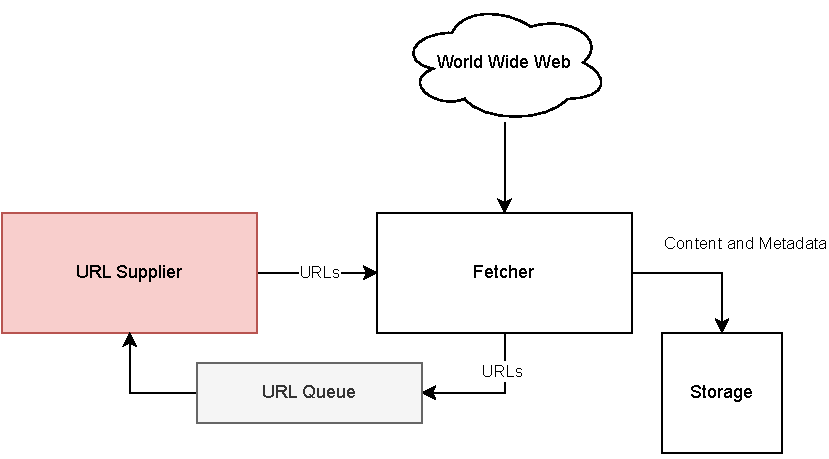
\includegraphics[width=14cm]{images/40_concept/HighLevelArch.pdf}
    \caption[Übersicht der Web-Crawler Basisarchitektur]{Übersicht der Web-Crawler Basisarchitektur bestehend aus URL-Supplier, Fetcher, URL-Queue sowie Storage.}
    \label{fig:architecture-general}
\end{figure}

Dieses grundlegende Prinzip basiert auf mehreren Komponenten, die miteinander interagieren. Der schematisch dargestellte \textbf{\textit{''URL-Supplier''}} führt die initiale Versorgung von Start-URLs durch, welche dann vom \textbf{\textit{''Fetcher''}} übernommen werden – dem Softwarebaustein, der den Download und das Verarbeiten des Inhalts durchführt. Unter Verarbeitung versteht man oft eine Filterung der URLs, bevor sie an eine weitere Komponente weitergegeben werden. Die abgerufenen Daten werden daraufhin in einer Datenbank gespeichert. Durch eine Auswertung des Inhalts, den der \textbf{\textit{''Fetcher''}} heruntergeladen hat, werden URLs gemäß bestimmter Regeln extrahiert. Diese extrahierten URLs gelangen dann in die \textbf{\textit{''URL-Queue''}}, wo sie vom \textbf{\textit{''Supplier''}} erneut weiterverarbeitet werden. Somit entsteht ein geschlossener Prozess.

Auf Basis dieses schematischen Prinzips wird nun eine skalierbare und effiziente Lösung entwickelt, um die in Kapitel \ref{sec:problem} angeführte Problemstellung zu adressieren. In den nachfolgenden Abschnitten, insbesondere in Kapitel \ref{sec:cloudnative} und \ref{sec:aot}, wird ein konkretes Konzept ausführlich erörtert.
\section{Einbettung in die Cloud-native Landschaft} \label{sec:cloudnative}
Der Cloud-native-Ansatz und die 12-Faktor-App-Methode sind zwei Konzepte, die eng miteinander verbunden sind und die Entwicklung von Anwendungen für die Cloud unterstützen. Der Cloud-native-Ansatz bezieht sich auf die Entwicklung von Anwendungen, die speziell für den Betrieb in einer Cloud-Umgebung optimiert sind. 
Die \textit{\ac{CNCF}} definiert den Begriff \textit{''Cloud-Native''}, um die Kernprinzipien - Skalierbarkeit, lose Kopplung, Resilienz, Observability und Manageability - zu vermitteln:

\begin{spar}
\textit{Cloud native technologies empower organizations to build and run scalable applications in modern, dynamic environments such as public, private, and hybrid clouds. Containers, service meshes, microservices, immutable infrastructure, and declarative APIs exemplify this approach.~\parencite[][]{CNCF}}
\end{spar}


Die 12-Faktor-App-Methode hingegen stellt eine Sammlung von Prinzipien und bewährten Vorgehensweisen dar, die bei der Entwicklung von Cloud-nativen Anwendungen befolgt werden sollte~\parencite[vgl.][]{12Factor}.
Zusammengefasst beinhaltet die 12-Faktor-App-Methode folgende Charakteristiken: 

\begin{spar}
\textit{Suitable to be deployed on cloud platforms, Scalable by design, Portable across systems, Enablers of continuous deployment and agility.~\parencite[][S. 36]{vitale}}
\end{spar}

Die skizzierten Prinzipien können in einer Web-Crawling Architektur ebenso Anwendung finden. In den nachfolgenden Abschnitten werden diese Prinzipien ausführlich behandelt und in den spezifischen Kontext des Web-Crawling eingebunden.

\subsection{Softwarearchitekturen in verteilten Systemen} \label{subsec:monoservmicro}
Wenn das Ziel darin besteht, eine Anwendung in eine Cloud-native Umgebung zu integrieren, um die Vorteile dieses Ansatzes voll auszuschöpfen, wird es früher oder später erforderlich sein, sich mit der Frage auseinanderzusetzen, welcher geeignete Softwarearchitekturansatz in diesem spezifischen Kontext am besten geeignet ist. In diesem Werk werden insbesondere die folgenden Ansätze beleuchtet: \textbf{\acl{SOA}} sowie \textbf{Microservice-Architektur.}\newline\newline
\textbf{\acl{SOA}}\newline
Serviceorientierung beschreibt eine sogenannte Basisarchitektur und definiert laut dem Werk \citetitle{Gharbi_Koschel_Rausch_Starke_2023}~\parencite[vgl.][]{Gharbi_Koschel_Rausch_Starke_2023}{}{} verteilte sowie lose gekoppelte Dienste. Diese Dienste stellen Schnittstellen bereit, über die Interaktionen ausgeführt werden können. Diese Interaktionen sollten in Form eines Vertrags zwischen dem Dienstanbieter und dem Dienstnutzer erfolgen. Diese Services sind eigenständige, wiederverwendbare Softwarekomponenten, die spezifische Funktionen bereitstellen. Sie ermöglichen eine Modularisierung und fördern die Wiederverwendbarkeit und Austauschbarkeit, da eine klar definierte Schnitstelle zwischen den Vertragspartnern existiert.\newline\newline
\textbf{Microservice-Architektur}\newline
    Die Microservice-Architektur ist laut \citetitle{Wolff_2018}~\parencite[vgl.][S. 6]{Wolff_2018} eine weitere Herangehensweise an die Entwicklung von Softwareanwendungen, bei der eine Anwendung in kleinere, unabhängige Dienste (Microservices) aufgeteilt wird. Der zuvor beleuchtete Ansatz der Serviceorientierung dient als Grundlage dafür. Jeder Microservice ist für einen klar definierten Teil der Funktionalität verantwortlich und kann eigenständig entwickelt, bereitgestellt und skaliert werden.

In der Arbeit von \citetitle{Wolff_2018}~\parencite[vgl.][S. 14-17]{Wolff_2018} werden die Vor- und Nachteile von Microservices umfassend diskutiert. Im nachstehenden Absatz werden die Schlüsselaspekte dieser Diskussion extrahiert und kurz erläutert. Darauf folgt eine detaillierte Analyse dieser Aspekte speziell im Rahmen des Web-Crawlings, wie in Abschnitt \ref{subsec:microservicekontextcrawler} näher ausgeführt wird.

    \textbf{Vorteile von Microservices:}
    \begin{itemize}
      \item \textbf{Getrennte Datenhaushalte:} Jeder Microservice verwaltet seine eigenen Daten, was die Änderbarkeit der Software erleichtert.
            
      \item \textbf{Flexibilität bei der Technologiewahl:} Jeder Microservice kann in einer anderen Technologie implementiert werden.

      \item \textbf{Unabhängige Skalierbarkeit:} Microservices ermöglichen eine gezielte Skalierung spezifischer Dienste, was die Ressourcennutzung effizienter macht.


    \end{itemize}
    
    \textbf{Nachteile von Microservices:}
    \begin{itemize}
      \item \textbf{Erhöhte Systemkomplexität:} Die Nutzung verschiedener Technologien erhöht die Gesamtkomplexität des Systems.
      
      \item \textbf{Verwundbarkeit in verteilten Systemen:} Microservices sind anfälliger\newline für Netzwerk- und Serverausfälle.
      
      \item \textbf{Architektonische Herausforderungen:} Die Aufteilung in Microservices kann zu unbeabsichtigten Abhängigkeiten führen.
    \end{itemize} 



\subsection[Analyse Microservice im Anwendungskontext]{Analyse Architekturmuster Microservice im Anwendungskontext}\label{subsec:microservicekontextcrawler}
Nachdem einige relevante Vor- und Nachteile von Microservices, basierend auf das Werk  \citetitle{Wolff_2018}~\parencite[vgl.][S. 14-17]{Wolff_2018}, betrachtet wurden, richtet sich der Fokus nun auf die Anwendung dieser Architektur im Bereich des Web-Crawlings, insbesondere im Hinblick auf die Skalierungseffizienz. Dieser Abschnitt konzentriert sich auf die Merkmale der Microservice-Architektur, die direkt die Skalierbarkeit und die damit verbundenen Herausforderungen beeinflussen. In den folgenden Abschnitten wird untersucht, wie diese spezifischen Eigenschaften von Microservices die Leistungsfähigkeit und Effizienz im Kontext des Web-Crawlings verbessern oder beeinträchtigen können.


\textbf{Loose Kopplung einzelner Services im Kontext von Web-Crawling}

Loose Kopplung stellt ein fundamentales Konzept innerhalb der\newline Microservice-Architektur dar, das im Bereich des Web-Crawlings eine zentrale Rolle einnimmt. Diese Eigenschaft ermöglicht es, diverse Aufgaben, die während des Crawling-Prozesses entstehen, flexibel zu managen.

Indem die Komponenten des Web-Crawling-Prozesses, wie das Abrufen von Webseiten, das Parsen von Inhalten und die Datenextraktion, in unabhängigen Microservices implementiert werden, erhöht sich die Autonomie jeder Komponente. Diese Modularität fördert nicht nur die Wartbarkeit und Fehlertoleranz durch die Isolation von Störungen in einzelnen Komponenten, sondern trägt auch zur Systemresilienz bei, indem es die Auswirkungen von Ausfällen minimiert. Dies ist besonders relevant in Umgebungen, in denen die Interaktion mit einer Vielfalt von Webseiten unvorhersehbare Fehler generieren kann.

\textbf{Unabhängige Skalierbarkeit im Kontext von Web-Crawling}

Unabhängige Skalierbarkeit, ein weiteres zentrales Prinzip der \newline Microservice-Architektur, ist im Web-Crawling essentiell. Diese Fähigkeit, einzelne Microservices bedarfsorientiert zu skalieren, ohne andere Systemkomponenten zu beeinträchtigen, ist entscheidend für die effiziente Ressourcen- und Leistungsverwaltung. Spezifische Dienste, verantwortlich für Crawling, Parsen oder Datenextraktion, können entsprechend den vorliegenden Anforderungen angepasst werden, was eine flexible Reaktion auf dynamische Lastsituationen ermöglicht.

\textbf{Zusammenspiel von loser Kopplung und unabhängiger Skalierbarkeit}

Die Integration von loser Kopplung und unabhängiger Skalierbarkeit in der Architektur von Web-Crawling-Systemen schafft signifikante Vorteile. Durch die lose Kopplung operieren Microservices als selbstständige Einheiten, was eine Prämisse für deren unabhängige Skalierung bildet.

Beispielsweise ermöglicht es die Architektur, den für das Parsen zuständigen Microservice separat zu skalieren, sollte dieser aufgrund eines erhöhten Datenaufkommens oder komplexer Inhaltsstrukturen unter Last stehen, unabhängig von anderen Services wie Datenextraktion oder Speicherung. So bleibt die Gesamtperformance des Crawling-Systems stabil, selbst wenn einzelne Komponenten spezifischen Herausforderungen gegenüberstehen.

\subsection{Eventbasierte vs Synchrone Inter-Service-Kommunikation}\label{subsec:eventdriven}
Im nachfolgenden Abschnitt erfolgt eine vergleichende Analyse zwischen eventbasierter und synchroner Kommunikation bei Services, welche das Ziel verfolgen, eine theoretische Grundlage für die weitere Konzeptionierung zu etablieren.

Eventbasierte Kommunikation in verteilten Systemen benötigt zwei Hauptkomponenten für den Nachrichtenaustausch zwischen Diensten. Die folgende Definition der Komponenten basiert auf dem Werk \citetitle{vitale}~\parencite[vgl.][]{vitale}{}{}.

\begin{enumerate}
    \item \textbf{Message-Broker}: vermittelt Nachrichten zwischen Sendern und Empfängern
    \item \textbf{Übertragungsprotokoll}: regelt die Datenübertragung zwischen\newline Sendern und Empfängern
\end{enumerate}

Die Kombination eines Message-Brokers mit einem dedizierten Übertragungsprotokoll ermöglicht asynchrone Kommunikation. Dabei müssen Anfragen und Antworten nicht sequenziell verarbeitet werden, sondern können unabhängig und basierend auf Verfügbarkeit bearbeitet werden. Die Vorteile dieses Ansatzes definiert \citetitle{vitale}~\parencite[vgl.][]{vitale}{}{} wie folgt:

 \begin{itemize}
  \item \textbf{Entkopplung der Service-Prozesse:} Services sind nicht gezwungen, auf direkte Antworten zu warten, wodurch Verzögerungen minimiert werden. 
  \item \textbf{Erhöhte Fehlertoleranz:} Bei Ausfall eines Services werden Nachrichten in der Warteschlange gehalten und gehen nicht verloren.
  \item \textbf{Skalierbarkeit:} Die asynchrone Verarbeitung ermöglicht eine bessere Skalierbarkeit, da Services unabhängig und parallel arbeiten können, ohne durch Synchronisationsprobleme eingeschränkt zu werden.
\end{itemize}

\ac{AMQP}, ein weit verbreitetes Übertragungsprotokoll, bietet vor allem durch zuverlässige Nachrichtenübermittlung und Interoperabilität zwischen Plattformen signifikante Vorteile \parencite[vgl.][]{vitale}. Bei dieser spielen sogenannte \textbf{''Event-Producer''} sowie \textbf{''Event-Consumer''} eine zentrale Rolle. Der Producer, so definiert es auch \citeauthor{vitale}~\parencite[vgl.][]{vitale}, ist dafür zuständig, Nachrichten zu versenden, hingegen der Consumer Nachrichten entgegennimmt. Dabei agieren Producer und Consumer unabhängig voneinander und haben keine direkte Verbindung zueinander. Visualisiert wird dies in Abbildung \ref{fig:amqp}.  
 
\begin{figure}[H]
    \centering
    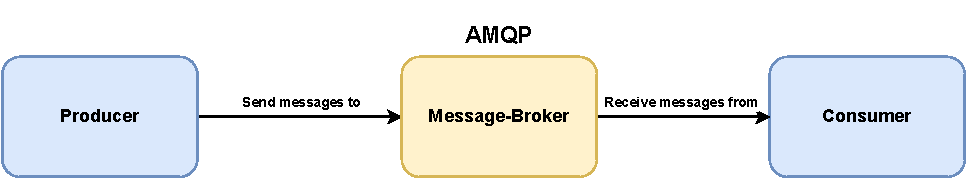
\includegraphics[width=14.5cm]{images/40_concept/AMQP.drawio.pdf}
    \caption[Visualisierung \acl{AMQP} Teilnehmer]{Visualisierung der Interaktion zwischen Event-Producer, Message-Broker und Event-Consumer in \ac{AMQP}~\parencite[vgl.][]{vitale}.}
    \label{fig:amqp}
\end{figure}
 Vor allem in Bezug auf die Zuverlässigkeit wird das verwendete Übertragungsprotokoll \ac{AMQP} relevant. So untersucht die Studie \textit{\citetitle{9023812}~\parencite[vgl.][]{9023812}{}{}} Alternativen, wie beispielweise \ac{MQTT}. Die Studie hebt hervor, dass \ac{AMQP} insbesondere in Szenarien mit hohen Anforderungen an die Zuverlässigkeit und Sicherheit der Datenübertragung überlegen ist. Die erwähnte Studie fokussiert sich zwar auf Anwendungen im Bereich ''Internet of Things'', jedoch lassen sich die Ergebnisse durchaus für weiterführende Forschung verwenden.

  Im Konzept dieser Arbeit sind Producer und Consumer zwei unterschiedliche Microservices. Ein RabbitMQ-Server fungiert als Message-Broker. Dieser Message-Broker wurde ausgewählt, da RabbitMQ sich durch die Verwendung von \ac{AMQP} auszeichnet. Eine empirische Analyse zwischen \ac{AMQP}-Message-Brokern bietet die Arbeit mit dem Titel \citetitle{9615705}~\parencite[vgl.][]{9615705}{}{}. In diesem wird RabbitMQ mit ActiveMQ, einer weiteren Implementierung eines Message-Brokers, verglichen. Durch diese Arbeit wird aufgezeigt, dass ActiveMQ zwar im Vergleich zum verwendeten RabbitMQ einen höheren Durchsatz an Nachrichten erlaubt, jedoch RabbitMQ eine geringere Latenz aufweist. Diese geringere Latenz wird in Abbildung \ref{fig:RABACTIVE} ersichtlich. Aufgrund der Optimierung der Durchlaufzeit des Prototyps wurde explizit ein Message-Broker mit einer geringen Latenz gewählt und der geringere Durchsatz mit einer optimierten Struktur des Nachrichten ausgeglichen. Dies ist in Kapitel \ref{subsec:eventbas} ersichtlich.

  \begin{figure}[H]
    \centering
    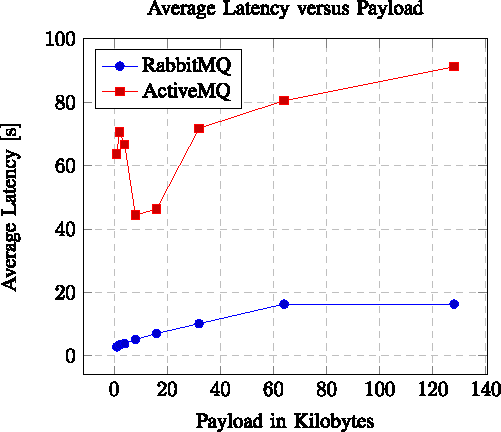
\includegraphics[width=10cm]{images/40_concept/Performance_Evaluation_of_Advanced_Message_Queuing_Protocol_AMQP_An_Empirical_Analysis_of_AMQP_Online_Message1_Brokers.pdf}
    \caption[Empirischer Vergleich zwischen ActiveMQ und RabbitMQ]{Empirischer Vergleich zwischen ActiveMQ und RabbitMQ in Bezug auf Latenz und Nachrichtengröße~\parencite[vgl.][]{9615705}{}{}.}
    \label{fig:RABACTIVE}
\end{figure}
Die Alternative zu einem asynchronen bzw. eventbasierten Ansatz wäre ein synchroner Datenaustausch, bei dem jede Anfrage eine unmittelbare Antwort erfordert, bevor der nächste Schritt erfolgen kann. Dies kann zu Engpässen führen, insbesondere in Systemen mit hoher Last, da der Verarbeitungsfluss durch die Antwortzeiten der einzelnen Services begrenzt wird. Im Gegensatz zum synchronen Datenaustausch führt ein eventbasiertes Verfahren jedoch zu einer erhöhten Komplexität, was unter anderem auch in Kapitel \ref{subsec:eventbas} verdeutlicht wird. In einem Web-Crawling Kontext, wo schnelle und effiziente Datenverarbeitung kritisch ist, könnte ein synchroner Ansatz aber die Leistungsfähigkeit des Gesamtsystems erheblich beeinträchtigen.

\subsection[Konzeptionierung Microservice im Anwendungskontext]{Konzeptionierung Architekturmuster Microservice im Anwendungskontext}
Die architektonische Übersicht in Abbildung \ref{fig:architecture} bietet einen umfassenden Überblick über die grundlegende Struktur der Softwareanwendung. Sie stellt die verschiedenen Hauptkomponenten und ihre Interaktionen dar. Diese Übersicht dient als Ausgangspunkt für die weitere Planung und Entwicklung der Anwendung und wird in diesem Kapitel genauer beschrieben.

\begin{figure}[H]
    \centering
    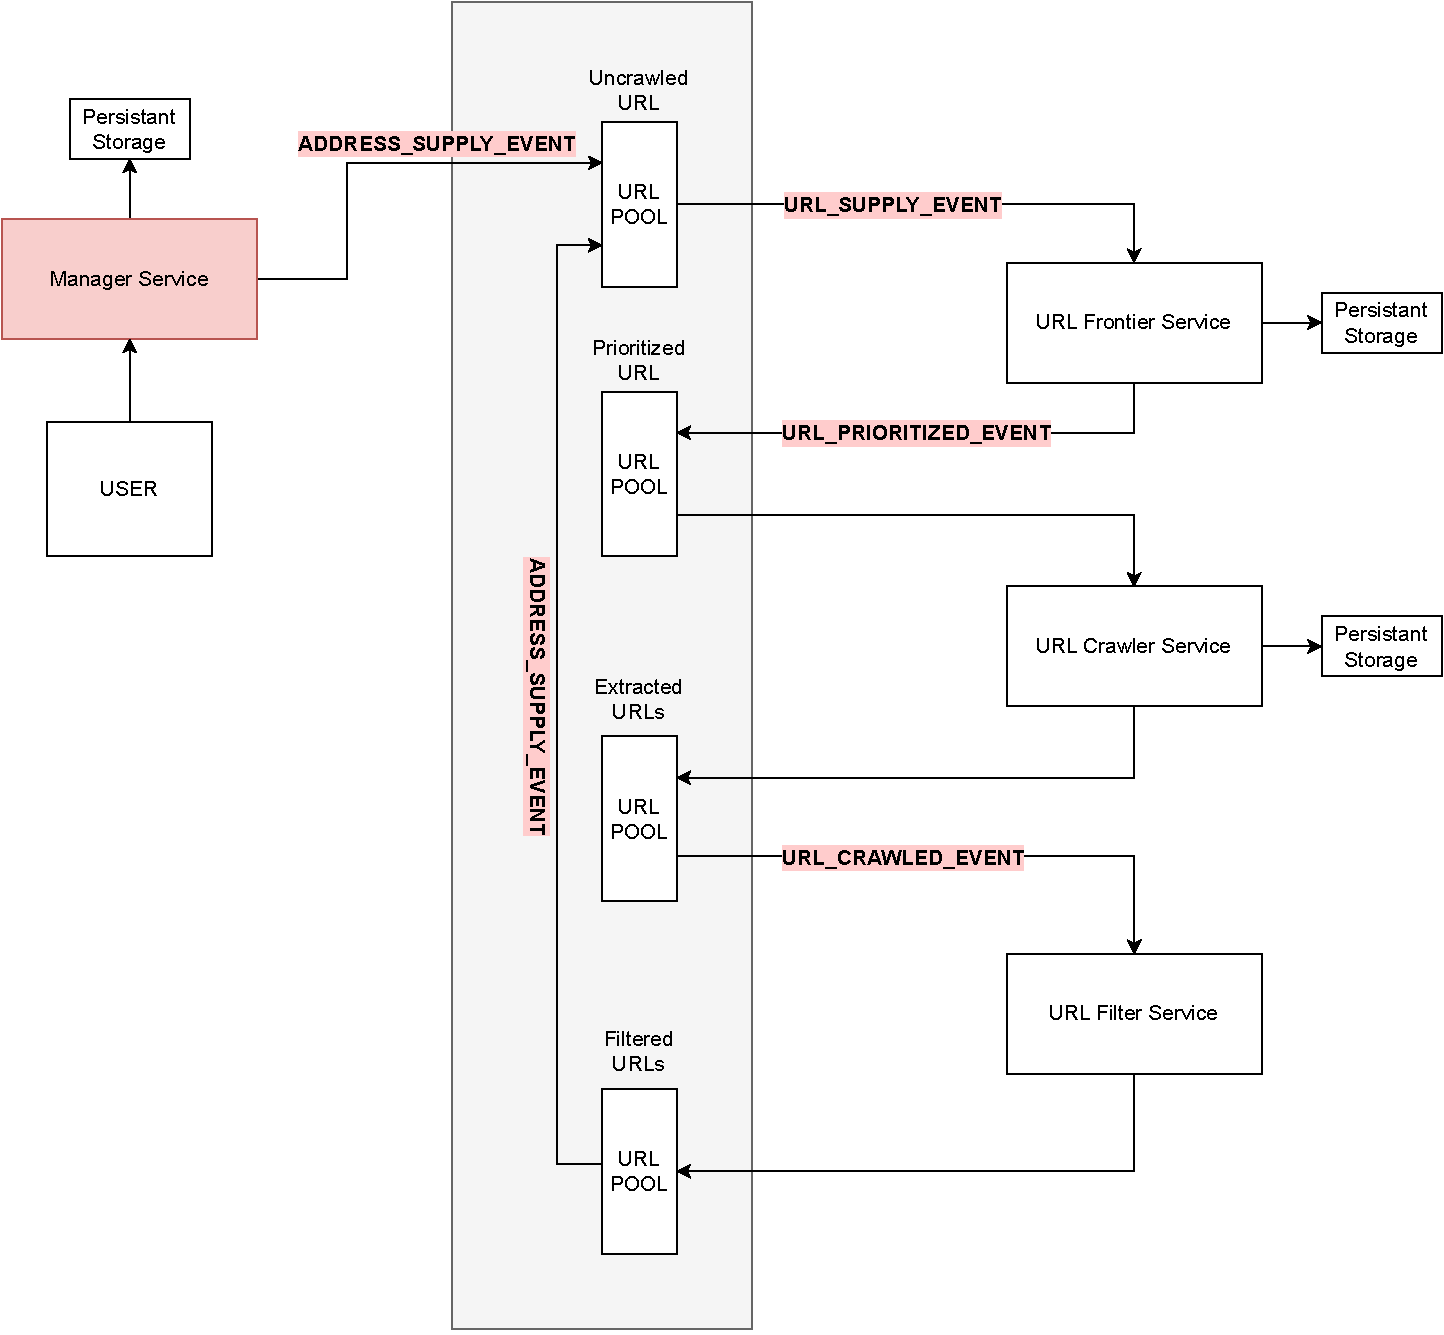
\includegraphics[width=14cm]{images/40_concept/microservice_conception.pdf}
    \caption[Visualisierung Web-Crawler Basisarchitektur]{Visualisierung der Aufteilung von einer Web-Crawler Basisarchitektur in Microservices samt Kommunikationsfluss.}
    \label{fig:architecture}
\end{figure}

Innerhalb der Architektur des Web-Crawlers nehmen sekundäre Services eine essenzielle Funktion ein. Diese Services verarbeiten eingehende Anfragen, die entweder direkt von Benutzern oder von anderen Servicekomponenten initiiert werden, und leiten die Ergebnisse entsprechend weiter. Ein kritisches Designprinzip, welches in Abschnitt \ref{subsec:microservicekontextcrawler} diskutiert wird, ist die lose Kopplung zwischen den einzelnen Microservices. Obwohl Interaktionen zwischen den Services sowohl möglich als auch erforderlich sind, ist eine direkte Abhängigkeit zu vermeiden. Aus diesem Grund wurde, wie in Abschnitt \ref{subsec:eventdriven} beschrieben, RabbitMQ als robustes Werkzeug für die Kommunikation zwischen den Services ausgewählt. Dies ermöglicht eine effiziente und zuverlässige Interaktion und unterstützt somit die Skalierbarkeit.
\newpage
Aufbauend auf den in Kapitel \ref{sec:traditionalconcepts} besprochenen traditionellen Konzepten, wurden spezifische Microservices für den Web-Crawler definiert. Diese Microservices sind:

\begin{itemize}
    \item \textbf{Manager Service:} Dieser Service fungiert als zentrale Steuerungseinheit, koordiniert die Aktivitäten der anderen Services und überwacht den Gesamtzustand des Crawling-Prozesses.
    \item \textbf{Frontier Service:} Verantwortlich für die Verwaltung der Crawling-Frontier, speichert dieser Service Informationen über zu besuchende URLs und priorisiert sie entsprechend.
    \item \textbf{Crawler Service:} Dieser Service führt das eigentliche Crawling durch, indem er Webseiten abruft und deren Inhalte extrahiert.
    \item \textbf{Filter Service:} Er filtert und bereinigt die extrahierten Daten, um sicherzustellen, dass nur relevante und qualitativ hochwertige Informationen für die weitere Verarbeitung verwendet werden.
\end{itemize}

Jeder dieser Services ist für einen spezifischen Aspekt des Web-Crawlings zuständig und trägt eine entscheidende Funktion zum Gesamtsystem bei. Im folgenden Kapitel wird eine detaillierte Aufgabenbeschreibung der einzelnen Services gegeben, um ihre Funktion ersichtlich zu machen. In der Grafik werden die Messages explizit hervorgehoben, welche über den Message-Broker ein- und ausgehen.

\noindent\rule{\textwidth}{1pt}

\textbf{Konzeption Manager Service}\newline
\textbf{Message-Queue Output:} Seed-URLs\newline
\begin{figure}[H]
    \centering
    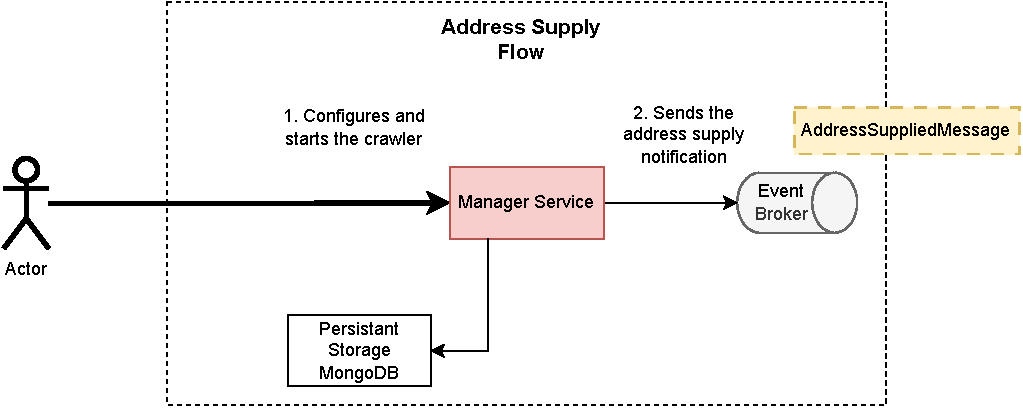
\includegraphics[width=14cm]{images/40_concept/ManagerService.drawio.pdf}
    \caption[Detailansicht des Manager Services]{Detailansicht des Manager Services samt Message-Queue-Interaktion sowie Darstellung der Benutzerschnitstelle.}
    \label{fig:ManagerService}
\end{figure}

Der Manager Service (siehe Abbildung \ref{fig:ManagerService}) ist für die Verwaltung von \newline Crawler-Konfigurationen zuständig und realisiert die entsprechenden Create-, Read-, Update- und Delete-Operationen. Dies ermöglicht es, Crawler-Konfigurationen zu erstellen, zu lesen, zu aktualisieren und zu entfernen. Zusätzlich ist der Manager Service dafür verantwortlich, Crawling-Prozesse zu initiieren und zu terminieren.

Die Konfigurationsdaten sowie der Status der Crawler werden in einer MongoDB-Datenbank persistiert. Die Wahl einer dokumentenbasierten Datenbank wie MongoDB ermöglicht Flexibilität in der Datenspeicherung, insbesondere durch die Fähigkeit, dynamisch neue Felder zu den Dokumenten hinzuzufügen, ohne die Struktur bestehender Datensätze zu beeinträchtigen.
Beim Start eines Crawlers generiert der Manager Service ein \textbf{\textit{AddressSuppliedMessage-Event}}, das über einen Event-Broker weitergeleitet wird. Dieses Ereignis enthält die initialen URLs für den Crawler, auch Seed-URLs genannt, und markiert den Beginn des Crawling-Prozesses. Der nachfolgende Service in der Verarbeitungskette, beispielsweise der Frontier Service, empfängt dieses Ereignis und setzt den Crawling-Prozess mit den bereitgestellten URLs fort.

Durch die beschriebene Funktionsweise agiert der Manager Service als zentrale Schnittstelle für die Steuerung und Überwachung der Crawler-Konfigurationen und -Status, wobei der Informationsfluss über definierte Ereignisse und die Speicherung von Zustandsinformationen in der Datenbank die Interoperabilität zwischen verschiedenen Services sicherstellt.\newline
\noindent\rule{\textwidth}{1pt}
\textbf{Konzeption Frontier Service}
\newline
\textbf{Message-Queue Input:} Seed-URLs bzw. gefilterte URLs\newline
\textbf{Message-Queue Output:} Priorisierte URLs\newline
\begin{figure}[H]
    \centering
    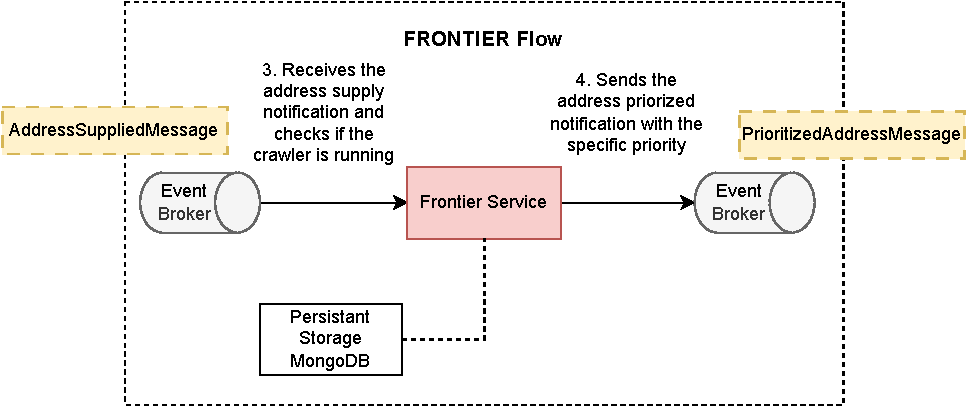
\includegraphics[width=14cm]{images/40_concept/FrontierService.drawio.pdf}
    \caption[Detailansicht des Frontier Services]{Detailansicht des Frontier Services samt Message-Queue-Interaktion.}
    \label{fig:FrontierService}
\end{figure}

Der Frontier Service (siehe Abbildung \ref{fig:FrontierService}) ist für die sogenannte \textbf{\textit{''Deduplication''}} der zu untersuchenden bzw. erhaltenen URL-Liste zuständig. Diese URL-Liste wurde entweder vom User als Seed-URL konfiguriert und vom Manager Service gesendet oder stammt von einem vorangegangenen Crawling-Prozess, bei dem der Filter Service die URLs normalisiert, gefiltert und weitergeleitet hat. Dieser Ansatz ist ein wichtiger Baustein und wird auch im bereits erwähnten Kapitel \textit{\nameref{sec:traditionalconcepts}} umgesetzt. So ist diese Funktion für einen vergleichbaren Prototypen essentiell. Er empfängt Seed-URLs bzw. extrahierte URLs vom Message-Broker, wie in Abbildung \ref{fig:FrontierService} dargestellt, und wählt diese für das Crawling aus. 

Der Frontier Service dient als primärer Knotenpunkt für den Beginn des Crawling-Prozesses und ist zuständig für die bereits erwähnte \textbf{\textit{''Deduplication''}} bzw. dem Aussortieren von URLs, die bereits verarbeitet wurden. Die Informationen zu bereits gecrawlten URLs werden in einer MongoDB gespeichert. Bereits gecrawlte URLs werden in diesem Vorgang nicht mehr gespeichert. Vor der Weiterleitung einer URL zum Crawling prüft der Frontier Service in dieser Datenbank, ob die betreffende URL bereits gecrawlt wurde. Sollte eine URL bereits verarbeitet worden sein, wird sie vom weiteren Crawling-Prozess ausgenommen, um Doppelarbeit zu verhindern. Der Frontier Service trägt somit die Verantwortung, sicherzustellen, dass keine URL mehrfach gecrawlt wird, und kann gegebenenfalls den Crawling-Vorgang für bereits analysierte Webseiten erneut initiieren. Nach dieser \textbf{\textit{''Deduplication''}} werden diese an den Event-Broker weitergeleitet.

\noindent\rule{\textwidth}{1pt}

\textbf{Konzeption Crawler Service}
\newline
\textbf{Message-Queue Input:} Vom Frontier-Service priorisierte URLs \\
\textbf{Message-Queue Output:} Liste der ungefilterten URLs

\begin{figure}[H]
    \centering
    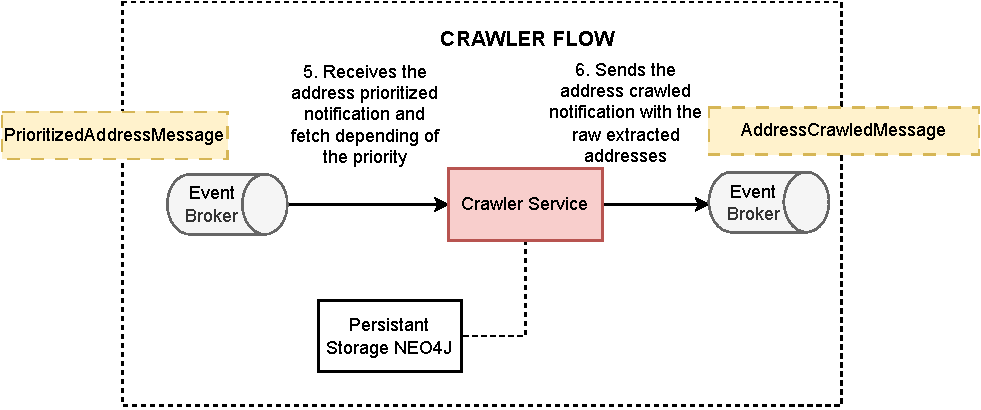
\includegraphics[width=14cm]{images/40_concept/CrawlerService.drawio.pdf}
    \caption[Detailansicht des Crawler Services]{Detailansicht des Crawler Services samt Message-Queue-Interaktion.}
    \label{fig:CrawlerService}
\end{figure}

Der Crawler Service (siehe Abbildung \ref{fig:CrawlerService}) ist ein entscheidender Bestandteil des \newline Crawling-Prozesses, der sich primär auf das Herstellen von Verbindungen zu Webservern und das Extrahieren von URLs konzentriert. 

Die primäre Funktion des Crawler Service ist das Etablieren von Verbindungen zu den Webservern der bereitgestellten URLs und das Abrufen der Webseiteninhalte. Dabei werden Techniken wie das Konfigurieren von Request-Headern, das Festlegen von Timeouts und das Implementieren von Wiederholungsmechanismen bei Verbindungsfehlern angewandt, um eine effiziente und fehlerresistente Datenakquisition zu gewährleisten.

Nach dem Herunterladen der Webseiteninhalte folgt die Analyse und das Extrahieren von URLs aus dem erhaltenen Webinhalt. Diese extrahierten URLs werden in einer strukturierten Nachricht, der \textbf{\textit{AddressCrawledMessage}}, gesammelt und für den nächsten Verarbeitungsschritt, beispielsweise dem Filter-Service, zur Verfügung gestellt.

Zudem ist der Crawler Service für die Persistenz der gewonnenen Daten zuständig. Die extrahierten URLs werden in einer Neo4j-Datenbank gesichert. Innerhalb dieser Graph-Datenbank werden die Webseiten als Knoten abgebildet und über Edges mit anderen gecrawlten Webseiten vernetzt, was die Analyse der Webstruktur ermöglicht und die Abfrageeffizienz steigert.

Der Manager Service bietet ein Konfigurationsobjekt, genannt \textit{\textbf{Actions}}, für die Indexierung der durch den Crawler Service erfassten Daten einer Webseite. Dieses Konfigurationsobjekt ermöglicht die Definition spezifischer Regeln, die festlegen, unter welchen Bedingungen ein bestimmter Index einer in der Datenbank gespeicherten Entität zugewiesen wird. Eine solche Aktion kann beispielweise einen Index auf eine Entität setzen, wenn eine bestimmte Zeichenfolge im Inhalt einer Webseite gefunden wird. In diesem Fall weist der Crawler Service der betreffenden Entität einen Index zu, um sie entsprechend zu markieren.

\noindent\rule{\textwidth}{1pt}
\newpage
\textbf{Konzeption Filter Service} \newline
\textbf{Message-Queue Input:} Liste der ungefilterten URLs\\
\textbf{Message-Queue Output:} Liste der gefilterten URLs

\begin{figure}[H]
    \centering
    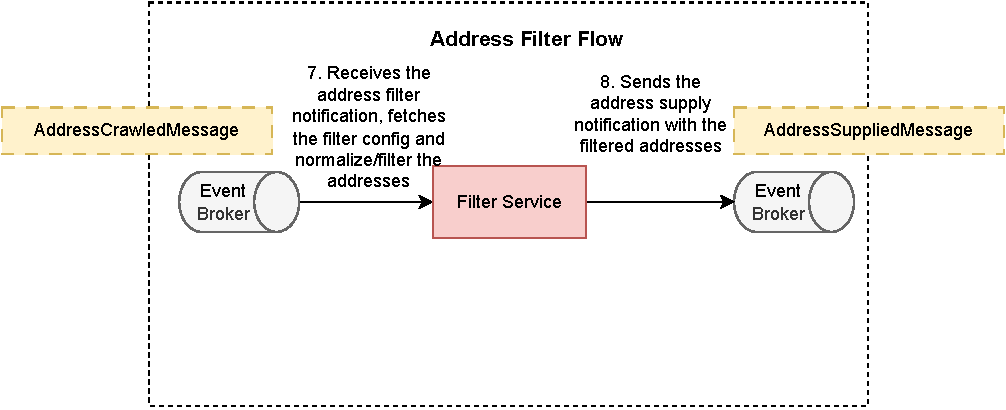
\includegraphics[width=14cm]{images/40_concept/FilterService.drawio.pdf}
    \caption[Detailansicht des Filter Services]{Detailansicht des Filter Services samt Message-Queue-Interaktion.}
    \label{fig:FilterService}
\end{figure}

Der Filter Service (siehe Abbildung \ref{fig:FilterService}) ist für die Normalisierung und Filterung der vom Crawler Service bereitgestellten URLs zuständig. Er transformiert die ungefilterten URLs in ein einheitliches Format und wendet festgelegte Filterkriterien an, um sicherzustellen, dass nur relevante Adressen für den weiteren Verarbeitungsprozess selektiert werden.

Im Normalisierungsprozess werden URLs gemäß definierten Regeln umgewandelt, um Konsistenz zu erreichen. Diese Normalisierung ist entscheidend, um eine effiziente Weiterverarbeitung durch andere Services im System zu gewährleisten.

Der anschließende Filterungsprozess prüft jede URL anhand einer konfigurierbaren Menge von Regeln und Kriterien. Diese Regeln können die Einschränkung auf bestimmte Domänen, Pfade oder Parameter beinhalten. URLs, die diesen Filterkriterien nicht entsprechen, werden eliminiert. Die entsprechende Filterkonfiguration wird durch den Manager-Service vorgegeben.

Abschließend werden die qualifizierten, gefilterten URLs an den Frontier Service übergeben, wodurch der Crawling-Zyklus erneut initiiert wird. Dieser Prozess stellt sicher, dass der Crawler nur auf URLs fokussiert, die den spezifischen Anforderungen des Systems entsprechen.


\section{Konzept Ahead-of-Time-Kompilierung} \label{sec:aot}
Das folgende Kapitel widmet sich eingehend dem Verständnis und der Anwendung von \acl{AOT}. Zunächst wird eine klare Definition der \acl{JIT} präsentiert, um ein solides Fundament für die nachfolgenden Diskussionen zu schaffen. Anschließend erfolgt eine umfassende Gegenüberstellung mit der \acl{AOT}, die es ermöglicht, die charakteristischen Merkmale und Vorteile beider Kompilierungsstrategien detailliert zu beleuchten. Den Abschluss bildet eine Erörterung darüber, wie die \acl{AOT} gezielt im Bereich des Web-Crawlings eingesetzt werden kann.
 \subsection{Definition von Just-in-time im Kontext JRE}
 Zu Beginn der Konzeptionierung von \ac{AOT} in den Anwendungskontext sollte auch definiert werden, auf welcher Basis man diesen Ansatz aufsetzen will. Eine Definition lässt sich beispielsweise gut durch die Programmiersprache Java formulieren, welche in späterer Folge für die Implementierung verwendet wird. Die Hochsprache Java erlangte unter anderem deshalb breite Akzeptanz, weil es durch das \ac{JRE} eine plattformübergreifende Ausführung ermöglichte. Entwickler/innen können ihren Code einmal schreiben und diesen überall ausführen, unabhängig vom Betriebssystem. Das Ziel wurde folgendermaßen definiert: \textit{''write them once, run them everywhere''~\parencite[vgl.][]{Gosling2023Java}.} Dieser Ansatz lässt sich bei weiteren objektorientierten Programmiersprachen beobachten, beispielsweise im .NET Framework die \textit{\ac{CLR}}.  

Durch die Kompilierung gemäß dem Java-Standard \parencite[vgl.][]{Lindholm2023JavaVM}, bei der der Java-Compiler Bytecode statt direktem Maschinencode erzeugt, wird eine plattformübergreifende Ausführung erzielt. Die Ausführung des Bytecodes übernimmt die \ac{JVM}, welche in Abbildung \ref{fig:JVMAOT} dargestellt wird.
 
 \begin{figure}[H]
    \centering
    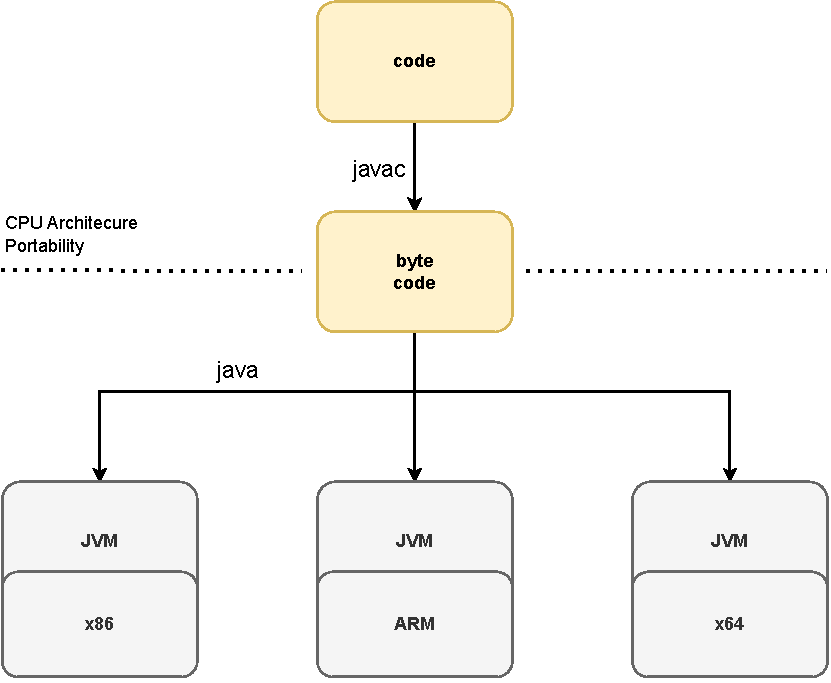
\includegraphics[width=12cm]{images/40_concept/JVM.pdf}
    \caption[Schematische Darstellung des Java-Kompilierungs- und Ausführungsprozesses]{Schematische Darstellung des Java-Kompilierungs- und Ausführungsprozesses~\parencite[vgl.][]{Lindholm2023JavaVM}.}
    \label{fig:JVMAOT}
\end{figure}
Die Bedeutung dieser Aussage wird durch eine Definition im JVM-Standard \citetitle{Lindholm2023JavaVM}~\parencite[vgl.][]{Lindholm2023JavaVM} verdeutlicht, die die essentiellen Prinzipien der Plattformunabhängigkeit von Programmcode betont:
 
 \begin{spar}
 \textit{The Java Virtual Machine knows nothing of the Java programming language, only of a particular binary format, the class file format. A class file contains Java Virtual Machine instructions (or bytecodes) and a symbol table, as well as other ancillary information. \parencite{Lindholm2023JavaVM}}
 \end{spar}

Innerhalb der Ausführungsumgebung der \ac{JVM} erfolgt die Verarbeitung des generierten Bytecodes. Dies wird in Abbildung \ref{fig:JVMEXEC} veranschaulicht.
\newline
 \begin{figure}[H]
    \centering
    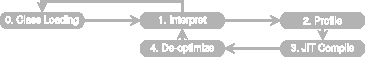
\includegraphics[width=12cm]{images/40_concept/path127.pdf}
    \caption[Darstellung des Ausführungszyklus innerhalb der \ac{JVM}]{Darstellung des Ausführungszyklus innerhalb der \ac{JVM}~\parencite[vgl.][]{9678709}{}{}.}
    \label{fig:JVMEXEC}
\end{figure}
Diese Verarbeitung beinhaltet das Laden der Class-Files, welche den Bytecode beinhalten, und dessen Transformation in Machine-Code. Ein sogenannter ''Interpreter'' ist für die Interpretation der Byte-Code-Instructions zuständig und wandelt diese in ausführbare Machine-Code-Instructions um~\parencite{Lindholm2023JavaVM}.

Die \ac{JVM} implementiert einen Optimierungsprozess während der Konvertierung des Bytecodes durch den \ac{JIT}-Compiler. Dazu nutzt die \ac{JVM} ein Verfahren namens \textit{Profiling}, um zu identifizieren, welche Teile des Codes beispielweise häufig interpretiert werden. Die Relevanz dieses Profiling-Mechanismus wird in \textit{\citetitle{9678709}} erläutert:

\begin{spar}
\textit{The JIT compiler cannot perform sophisticated code analysis and code optimization} when JVM does not have a complete picture of a Java method. JVM thus accumulates method execution counters and collects various method profiling data during interpretation.~\parencite[][]{9678709}{}{}
\end{spar}

Basierend auf dem Profiling-Prozess wird der sogenannte \textit{''Hot-Code''} direkt in nativen Code kompiliert und optimiert. Diese Vorgehensweise eliminiert die Notwendigkeit für eine wiederholte Übersetzung von Bytecode-Instructions in Machine-Code-Instructions durch den Interpreter, indem sie direkten Zugriff auf den durch den JIT-Compiler optimierten Machine-Code ermöglicht~\parencite{Lindholm2023JavaVM}.


\subsection{Limitierungen von Just-in-time im Kontext JRE}

In der Domäne der \ac{JVM} basierten Anwendungen manifestieren sich spezifische Herausforderungen. Initialisierungszeit und Speicherplatzbedarf sind mitunter Probleme, mit denen man konfrontiert ist. Aus diesen Herausforderungen forumliert sich die Hypothese aus Kapitel \ref{subsec:hypothesis:ressource}. Traditionelle Anwendungssysteme charakterisieren sich durch erhebliche Latenzen bei der Initialisierung. Dies untermauert auch das Werk \textit{\citetitle{9678709}}. Dieses ergründet diese durchaus langen Latenzzeiten mit folgender Aussage:

\begin{spar}
    \textit{Largescale Java applications usually have tens of thousands of Java classes or even more, which are packaged into thousands of JAR files. In practice, it can take minutes for those applications to start up before they are online and begin to process user requests.~\parencite[][]{9678709}{}{}}
\end{spar}

Demgegenüber steht die Anforderung, dass Anwendungen, welche den Prinzipien \newline Cloud-nativer Architekturen folgen, signifikant reduzierte Startzeiten aufweisen, ein markanter Kontrast zu den vormals üblichen, durchaus längeren Zeiträumen. Obwohl diese reduzierte Initialisierungszeit für eine Vielzahl von Anwendungsfällen als adäquat betrachtet wird, ergibt sich für Cloud-Architekturen, die eine quasi-instantane Verfügbarkeit erfordern, eine nicht zu vernachlässigende Problematik~\parencite[vgl.][]{12Factor}. 

 
 \subsection{Definition von Ahead-of-time und Anwendung mit GraalVM}
 Im Vergleich zu \ac{JIT} ist \ac{AOT} ein vollkommen anderer Ansatz. Die \acl{AOT} übersetzt Hochsprachencode in Machine-Code bevor das Programm ausgeführt wird, also während der Kompilierzeit. Dies steht im Kontrast zur \acl{JIT}, die Code erst während der Laufzeit kompiliert. AOT bereitet den Code so auf, dass er direkt ausführbar ist. 
 Spricht man nun über den Kontext in Java, bietet die GraalVM \parencite[vgl.][]{graalvm2023} eine Alternative zu vorhandenen JDKs. Dieser GraalVM Standard ist eine Ausprägung der OpenJDK und teil des OpenJDK's Graal Projektes. Dieses Projekt verfolgt grundsätzlich folgendes Ziel:

 \begin{spar}
 \textit{[...]designed to accelerate the execution of applications written in Java and other JVM languages.~\parencite{graalvm2023}}
 \end{spar}

 Als OpenJDK-Alternative soll dieser Ansatz laut \citetitle{graalvm2023}~\parencite[vgl.][]{graalvm2023} eine Steigerung der Effizienz sowie Leistung bringen. Der Graal-Compiler, welcher nun für die Kompilierung von Applikationscode zuständig ist, bietet zwei Betriebsmodi: vorab kompilierter Maschinencode \textbf{\textit{(''libgraal'')}} oder dynamisch ausgeführter Java-Bytecode \textbf{\textit{(''jargraal'')}}. Der GraalVM Native-Image-Builder, welcher eine direkte Kompilierung von Java-Anwendungen in Maschinencode durchführt, ist für ersteren Betriebsmodi zuständig. Das Ergebnis ist ein natives Ausführungsformat, das sämtlichen für die Ausführung notwendigen Maschinencode enthält. Dieser Maschinencode muss nun nicht mehr in einer \ac{JVM} interpretiert und in Maschinencode umgewandelt werden, da dieser Vorgang bereits zu Kompilierzeit erfolgt.

\subsection{Evaluierung der \acl{AOT}}
Die \ac{AOT}-Kompilierung in Java bietet eine Reihe von Vorteilen aber bringt auch Herausforderungen mit sich. Diese werden im folgenden Abschnitt aufgezeigt.

 \textbf{Vorteile der \acl{AOT}}
\begin{enumerate}
    \item \textbf{Verbesserung der Laufzeitperformance:} \ac{AOT}-Kompilierung kann die Startzeit von Java-Anwendungen erheblich reduzieren, indem die Interpretation und Optimierung zur Laufzeit nicht mehr notwendig ist~\parencite[vgl.][]{9678709}.

     \item \textbf{Minimierung der ''Warm-Up''-Phase:} Mit \ac{AOT}-Artefakten erreicht man unmittelbar nach dem Start der Applikation die maximale Leistungsfähigkeit, ohne eine sogenannte ''Warm-Up''-Phase~\parencite[vgl.][]{9678709}. 
\end{enumerate}
 \textbf{Nachteile der \acl{AOT}-Kompilierung}
\begin{enumerate}
    \item \textbf{Verlust der Plattformunabhängigkeit:} Ein wesentlicher Nachteil von \ac{AOT}-Kompilierung ist der Verlust der Plattformunabhängigkeit. Im Unterschied zu \ac{JIT}-Compilern, die plattformübergreifenden Bytecode in Maschinencode umwandeln, produzieren \ac{AOT}-Compiler direkt plattformspezifischen Code. 
    
    \item \textbf{Längere Kompilierungszeiten:} Die Erstellung von \ac{AOT}-Artefakten kann länger dauern als die Erstellung mit \ac{JIT}-Kompilierung, da die gesamte Anwendung im Voraus kompiliert wird. Auf diesen Nachteil wird unter anderem auch in Kapitel \ref{chap:evaluation} eingegangen.

\end{enumerate}

\subsection{Integration in den Web-Crawling Kontext}

Die Implementierung der diskutierten Technologie im Rahmen von Web-Crawling Prozessen adressiert potenziell die Herausforderungen, die in Kapitel \ref{sec:problem} dargelegt wurden. Für Web-Crawling-Service-Instanzen ist eine effiziente Verarbeitung großer Datenmengen, wie sie in der Problemstellung beschrieben wird, essenziell. Dieser Prozess sollte möglichst ressourcenschonend sein. So ist dies eine vielversprechende Technik, um einige Probleme in diesem Kontext zu lösen.

Referenziert auf die Hypothese \ref{subsec:hypothesis:ressource} könnten in diesem Zusammenhang insbesondere die optimierten Startzeiten zu einer erheblichen Verbesserung führen.

Der Web-Crawling Prototyp wird nun auf diese Weise optimiert, um eine gezielte Aussage treffen zu können. Diese Implementierung ist in Kapitel \ref{sec:aotoptimizing} beschrieben.
\chapterend